
\subsection{Iteración 1}

El objetivo inicial de esta entrega era el de diseñar y crear todo el flujo que seguirá el juego. Teniendo en cuenta de que se pretende recrear un concurso televisivo, se va desarrollar una introducción que describa el concurso y presente las reglas al jugador, además de las fases que ocurrirán al principio y final de cada prueba, así como entre cada una de ellas. Finalmente, se añadirá un menú en el que se podrán cambiar los ajustes del juego, entre ellos: la dificultad, los tipos de pruebas que aparecerán, si el jugador está sentado o de pie, o si el jugador tendrá ayuda de una persona externa o no.

Este objetivo se ha visto alterado por pasar a disponer de un nuevo dispositivo de RV para el desarrollo, en este caso las gafas Meta Quest 2. Como se explica en la sección \textbf{Tecnología a usar} (\ref{sec:tecnologiaUsar}), este dispositivo es mucho más deseable para este proyecto, ya que permite prescindir de un ordenador externo al que conectar las gafas, del uso de estaciones base separadas para realizar el seguimiento del casco y los mandos, y al ser más reciente permite utilizar las bibliotecas más modernas para facilitar el desarrollo. Por estas razones, aún suponiendo un extra de carga de trabajo, se decide realizar el cambio de dispositivo, el cual se describe a continuación.


\subsubsection{Migración dispositivo VR}

El primer paso es crear una copia de seguridad en caso de haber alguna incompatibilidad. A continuación, se descarga la última versión del editor de Unity, en este caso se usará la versión 2023.1.9f1. Una vez instalada, abrimos el proyecto usando la nueva versión. Durante la migración de una versión a otra aparecen errores de y se recibe el aviso de que el proyecto puede no funcionar. Cuando se abre el proyecto aparece un nuevo aviso sobre varios paquetes que están obsoletos (\ref{fig:deprecated})




\begin{figure}
	\centering
	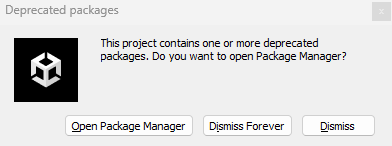
\includegraphics[width=0.7\textwidth]{04.Desarrollo/05.Entrega5/01.Iteracion5_1/00.Figuras/03.deprecated.png}
	\caption{Aviso sobre paquetes obsoletos.}
	\label{fig:deprecated}
\end{figure}


Tras desinstalar los paquetes obsoletos, en este caso tanto SteamVR, Zinnia y VRTK, se va a proceder a instalar las nuevas bibliotecas para Meta Quest 2, para ello se va a seguir la documentación oficial. \cite{DES_5_1_oculusSDK} El proceso a seguir es sencillo y consiste en importar el nuevo paquete OculusIntegration (versión 55 en este caso). No ha surgido ningún nuevo problema, la documentación es buena y muy visual, y un proceso similar ya se ha descrito en la \textbf{Entrega 1} (\ref{sec:Entrega1Iteracion1}), por lo que no voy a desarrollar mucho esta instalación.

Una vez instalada la nueva biblioteca, el siguiente paso es recuperar todas las funcionalidades que ya estaban desarrolladas para las HTC Vive anteriormente. Por suerte el SDK de integración de Oculus es muy completo y tiene ya implementado casi todo lo necesario. Usando el objeto OculusInteractionSampleRig (figura \ref{fig:sample_rig}), podemos añadir a la escena tanto la cámara como los controladores y todo lo necesario para el seguimiento y la interacción básica con el juego.

\begin{figure}
	\centering
	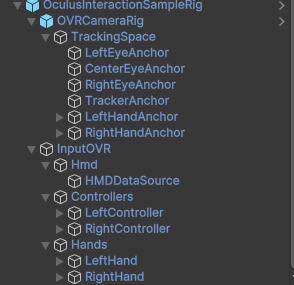
\includegraphics[width=0.7\textwidth]{04.Desarrollo/05.Entrega5/01.Iteracion5_1/00.Figuras/04.sample_rig.png}
	\caption{Jerarquía del objeto OculusInteractionSampleRig incluido con el SDK de Meta.}
	\label{fig:sample_rig}
\end{figure}


Para facilitar el uso del juego a personas con pocos conocimientos tecnológicos, se va a usar el seguimiento de manos proporcionado por el visor, de esta forma se proyecta en el juego una representación exacta de las manos de los usuarios y sus movimientos, como se puede ver en la figura \ref{fig:hand_tracking}.

\begin{figure}
	\centering
	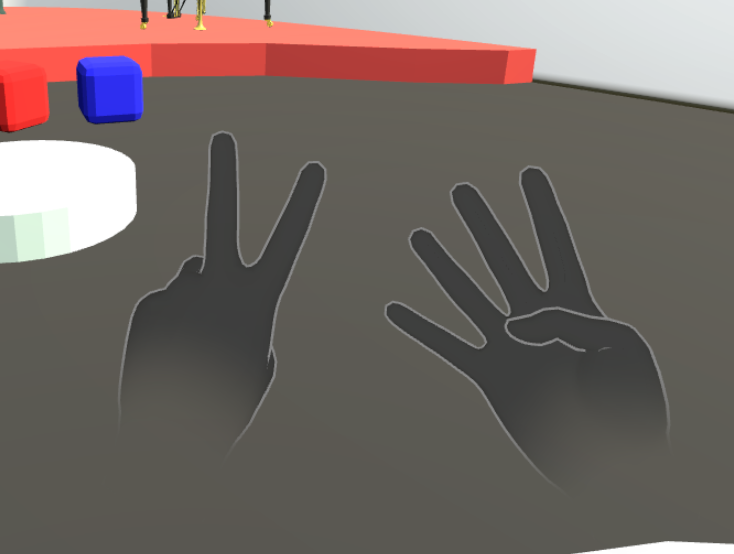
\includegraphics[width=0.7\textwidth]{04.Desarrollo/05.Entrega5/01.Iteracion5_1/00.Figuras/05.hand_tracking.png}
	\caption{Manos virtuales captadas usando el seguimiento de Meta Quest 2.}
	\label{fig:hand_tracking}
\end{figure}

A continuación es necesario añadir las posibles interacciones de las manos con el entorno, en este caso: coger y pulsar objetos y poder seleccionar elementos lejanos mediante un rayo. De nuevo, el SDK proporciona elementos ya configurados para estos casos. Solo es necesario añadirlos a la jerarquía según la figura \ref{fig:interactors}. En este caso se añaden tanto para las manos como para los mandos, en caso de desear utilizarlos.


\begin{figure}
	\centering
	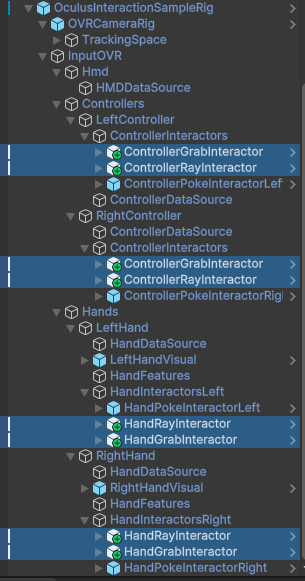
\includegraphics[width=0.7\textwidth]{04.Desarrollo/05.Entrega5/01.Iteracion5_1/00.Figuras/06.interactors.png}
	\caption{\textit{Interactors} que permiten coger, pulsar o lanzar rayos.}
	\label{fig:interactors}
\end{figure}

Finalmente, para que un objeto del juego pueda interactuar con el jugador, necesita nuevos scripts también proporcionados por el SDK, en este caso son: 

♠\begin{itemize}
	\item {\textit{Grabbable}: Permite que un objeto pueda ser cogido y define su comportamiento.}
	\item{\textit{Grab Interactable}: Permite que el elemento sea cogido con los mandos.}
	\item{\textit{Hand Grab Interactable}: Permite que el elemento sea cogido con las manos.}
	\item{\textit{Ray Interactable}: Permite lanzar un rayo sobre el objeto para interactuar con él.}
\end{itemize}


Tras estos pasos, la migración queda terminada y podemos comenzar a utilizar Meta Quest 2 y su seguimiento de manos en el proyecto. Aunque aún es necesario cambiar el funcionamiento de varias pruebas debido a cambios en las nuevas bibliotecas.


En concreto es necesario actualizar las zonas de \textit{snap} utilizadas en las pruebas de asociación, donde el jugador debe coger y colocar en plataformas distintos objetos, agrupándolos por categorías. Lo que se ha decidido hacer es reemplazar este sistema por otro más sencillo en el que un \textit{trigger} sobre la plataforma detecta los objetos que se introducen en él, comprobando si tienen o no la categoría deseada. El funcionamiento es muy similar al método anterior pero simplificado y eliminando el uso de la anterior biblioteca.














